\documentclass[aspectratio=169, 12pt]{beamer}

\usepackage{lmodern}
\usepackage{hyperref}
\usepackage{graphicx}
% \usepackage[authordate,backend=biber,doi=false,isbn=false,url=false]{biblatex-chicago}
% \addbibresource{my.bib}

\usepackage{amsmath}
\usepackage{amssymb}
\usepackage{amsthm}
\usepackage{bm}
\usepackage{bbm}
\usepackage{mathtools}
\setbeamertemplate{theorems}[numbered]
\newtheorem{thm}{Theorem}
\newtheorem{proposition}[thm]{Proposition}

\DeclareMathOperator*{\plim}{plim}
\DeclareMathOperator*{\var}{var}
\DeclareMathOperator*{\cov}{cov}

\newcommand{\indep}{\perp \!\!\! \perp}
\newcommand{\R}{\mathbb{R}}
\newcommand{\I}{\mathbbm{1}}
\newcommand{\argmax}{\mathop{\rm arg~max}\limits}
\newcommand{\argmin}{\mathop{\rm arg~min}\limits}

\usepackage{booktabs}
\usepackage{dcolumn}

\usepackage[group-separator={,}]{siunitx}
\usepackage{ctable}
\setupctable{captionsleft}

\usepackage{silence}
\WarningFilter{latexfont}{Font shape}
\WarningFilter{biblatex}{Patching footnotes failed}

\usetheme{Boadilla}
\usecolortheme{orchid}
\usefonttheme{professionalfonts}

\setbeamertemplate{section in toc}[sections numbered]
\setbeamertemplate{itemize item}[default]
\setbeamertemplate{itemize subitem}[square]
\setbeamertemplate{enumerate items}[default]
\setbeamertemplate{navigation symbols}{}
\setbeamertemplate{itemize/enumerate body begin}{\normalsize}
\setbeamertemplate{itemize/enumerate subbody begin}{\normalsize}
\setbeamertemplate{itemize/enumerate subsubbody begin}{\normalsize}
\setbeamerfont{title}{size=\large}
\setbeamerfont{institute}{size=\small}

\title[TMLE and DML]{Targeted minimum loss-based estimation and double/debiased machine learning}
\author[Konan Hara]{Konan Hara}
\institute[Arizona]{University of Arizona}
\date{July 25, 2022}
\begin{document}

	\begin{frame}[plain]
	\titlepage
	\end{frame}

	\begin{frame}
	\frametitle{References}
	\begin{itemize}
	\item ``Targeted Maximum Likelihood Learning'' by van der Laan \& Rubin (2006)
	\item ``\href{https://vanderlaan-lab.org/2019/12/24/cv-tmle-and-double-machine-learning/}{\underline{CV-TMLE and double machine learning}}'' in van der Laan's website
	\item ``Machine learning in the estimation of causal effects: targeted minimum loss-based estimation and double/debiased machine learning'' by D\'iaz (2020)
	\item ``Double/debiased machine learning for treatment and structural parameters'' Chernozhukov, Chetverikov, Demirer, Duflo, Hansen, Newey, \& Robins (2018)
	\item ``Locally Robust Semiparametric Inference with Debiased GMM'' by Chernozhukov, Escanciano, Ichimura, Newey, \& Robins (2022)
	\end{itemize}
	\end{frame}

	\begin{frame}
	\frametitle{Regularization Bias}
	\begin{itemize}
	\item Variables
	\begin{itemize}
	\item $Y$: outcome
	\item $D$: treatment indicator
	\item $X$: covariates
	\end{itemize}
	\item Observe $(y_i,d_i,x_i) \sim P_0 $ i.i.d. for $i=1,\dots,N $
	\item Easy to get $\sqrt{N}$-consistent $\theta_0$ if
	\begin{eqnarray*}
	Y = D\theta_0 + X^\top \beta_0 + U, E[U|X,D]=0, \beta_0 \in \R^p, \text{ where } p \text{ is small enough.}
	\end{eqnarray*}
	\item What happens if we apply lasso to the following model?
	\begin{eqnarray*}
	Y = D\theta_0 + X^\top \beta_0 + U, E[U|X,D]=0, \beta_0 \in \R^p, \text{ where } p \text{ is very large.}
	\end{eqnarray*}
	\end{itemize}
		
	\end{frame}


	\begin{frame}
	\frametitle{Regularization Bias}
	What happens if we apply ML prediction approach to the following model?
	\begin{eqnarray*}
	Y = D\theta_0 + g_0(X) + U, E[U|X,D]=0.
	\end{eqnarray*}
	\begin{enumerate}
	\item Start from a guess of $\theta_0 \Rightarrow \hat{\theta}^0 $
	\item Apply ML to predict $Y-D\hat{\theta}^0 $ using $X \Rightarrow \hat{g}^1(\cdot) $
	\item Regress $Y-\hat{g}^1(X) $ on $D \Rightarrow \hat{\theta}^1 $
	\item Iterate until convergence $\Rightarrow \hat{\theta}_0 $
	\end{enumerate}
	
	\end{frame}

	\begin{frame}
	\frametitle{Regularization Bias}
	\begin{figure}
	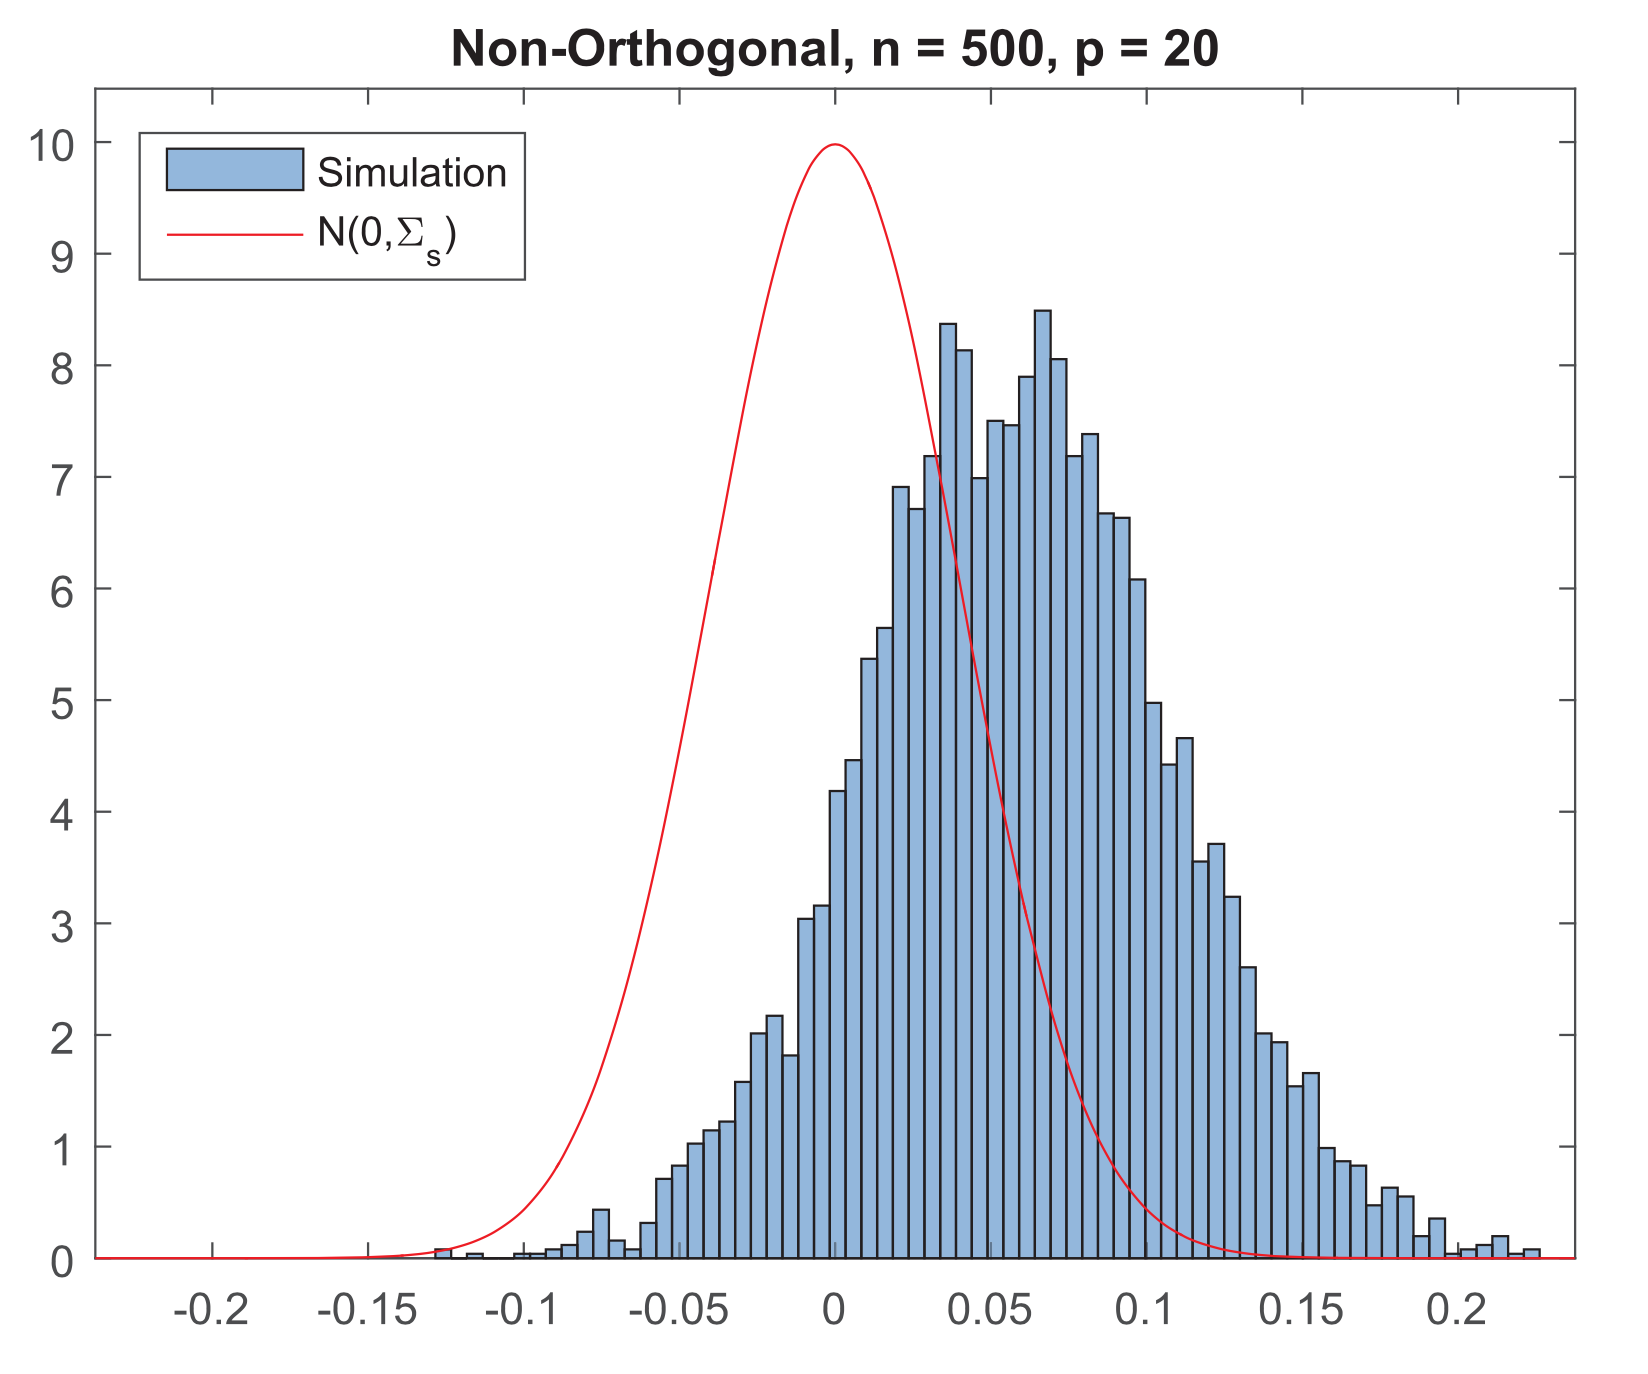
\includegraphics[width=0.6\textwidth]{fig/fig1a.png}
	\end{figure}

	\end{frame}
	
	\begin{frame}
	\frametitle{Frish-Waugh-Lowell Theorem}
	Consider
	\begin{eqnarray*}
	Y = D\theta_0 + X^\top \beta_0 + U, E[U|X,D]=0, \beta_0 \in \R^p, \text{ where } p \text{ is small enough.}
	\end{eqnarray*}
	$\theta_0$ can be consistently estimated by regressing
	\begin{itemize}
	\item residual of regression $Y$ on $X$
	\end{itemize}
	on
	\begin{itemize}
	\item residual of regression $D$ on $X$.
	\end{itemize}

	\end{frame}

	\begin{frame}
	\frametitle{Double/Debiased Machine Learning Estimator}
	What happens if we apply FWL-style estimation to the following?
	\begin{eqnarray*}
	Y = D\theta_0 + X^\top \beta_0 + U, E[U|X,D]=0, \beta_0 \in \R^p, \text{ where } p \text{ is very large.}
	\end{eqnarray*}
	\begin{enumerate}
	\item Apply lasso to predict $D$ by $X$, and collect the residual $\Rightarrow \hat{V} $
	\item Apply lasso to predict $Y$ by $X$, and collect the residual $\Rightarrow \hat{W} $
	\item Regress $\hat{W} $ on $\hat{V} \Rightarrow$ DML estimator $\hat{\theta}_0 $
	\end{enumerate}

	\end{frame}

	\begin{frame}
	\frametitle{Double/Debiased Machine Learning Estimator}
	Consider a more general situation:
	\begin{eqnarray*}
	Y = D\theta_0 + g_0(X) + U, E[U|X,D]=0.
	\end{eqnarray*}
	\begin{enumerate}
	\item Apply ML to predict $D$ by $X$, and collect the residual $\Rightarrow \hat{V} $
	\item Apply ML to predict $Y$ by $X$, and collect the residual $\Rightarrow \hat{W} $
	\item Regress $\hat{W} $ on $\hat{V} \Rightarrow$ DML estimator $\hat{\theta}_0 $
	\end{enumerate}

	\end{frame}

	\begin{frame}
	\frametitle{Double/Debiased Machine Learning Estimator}
	\begin{figure}
	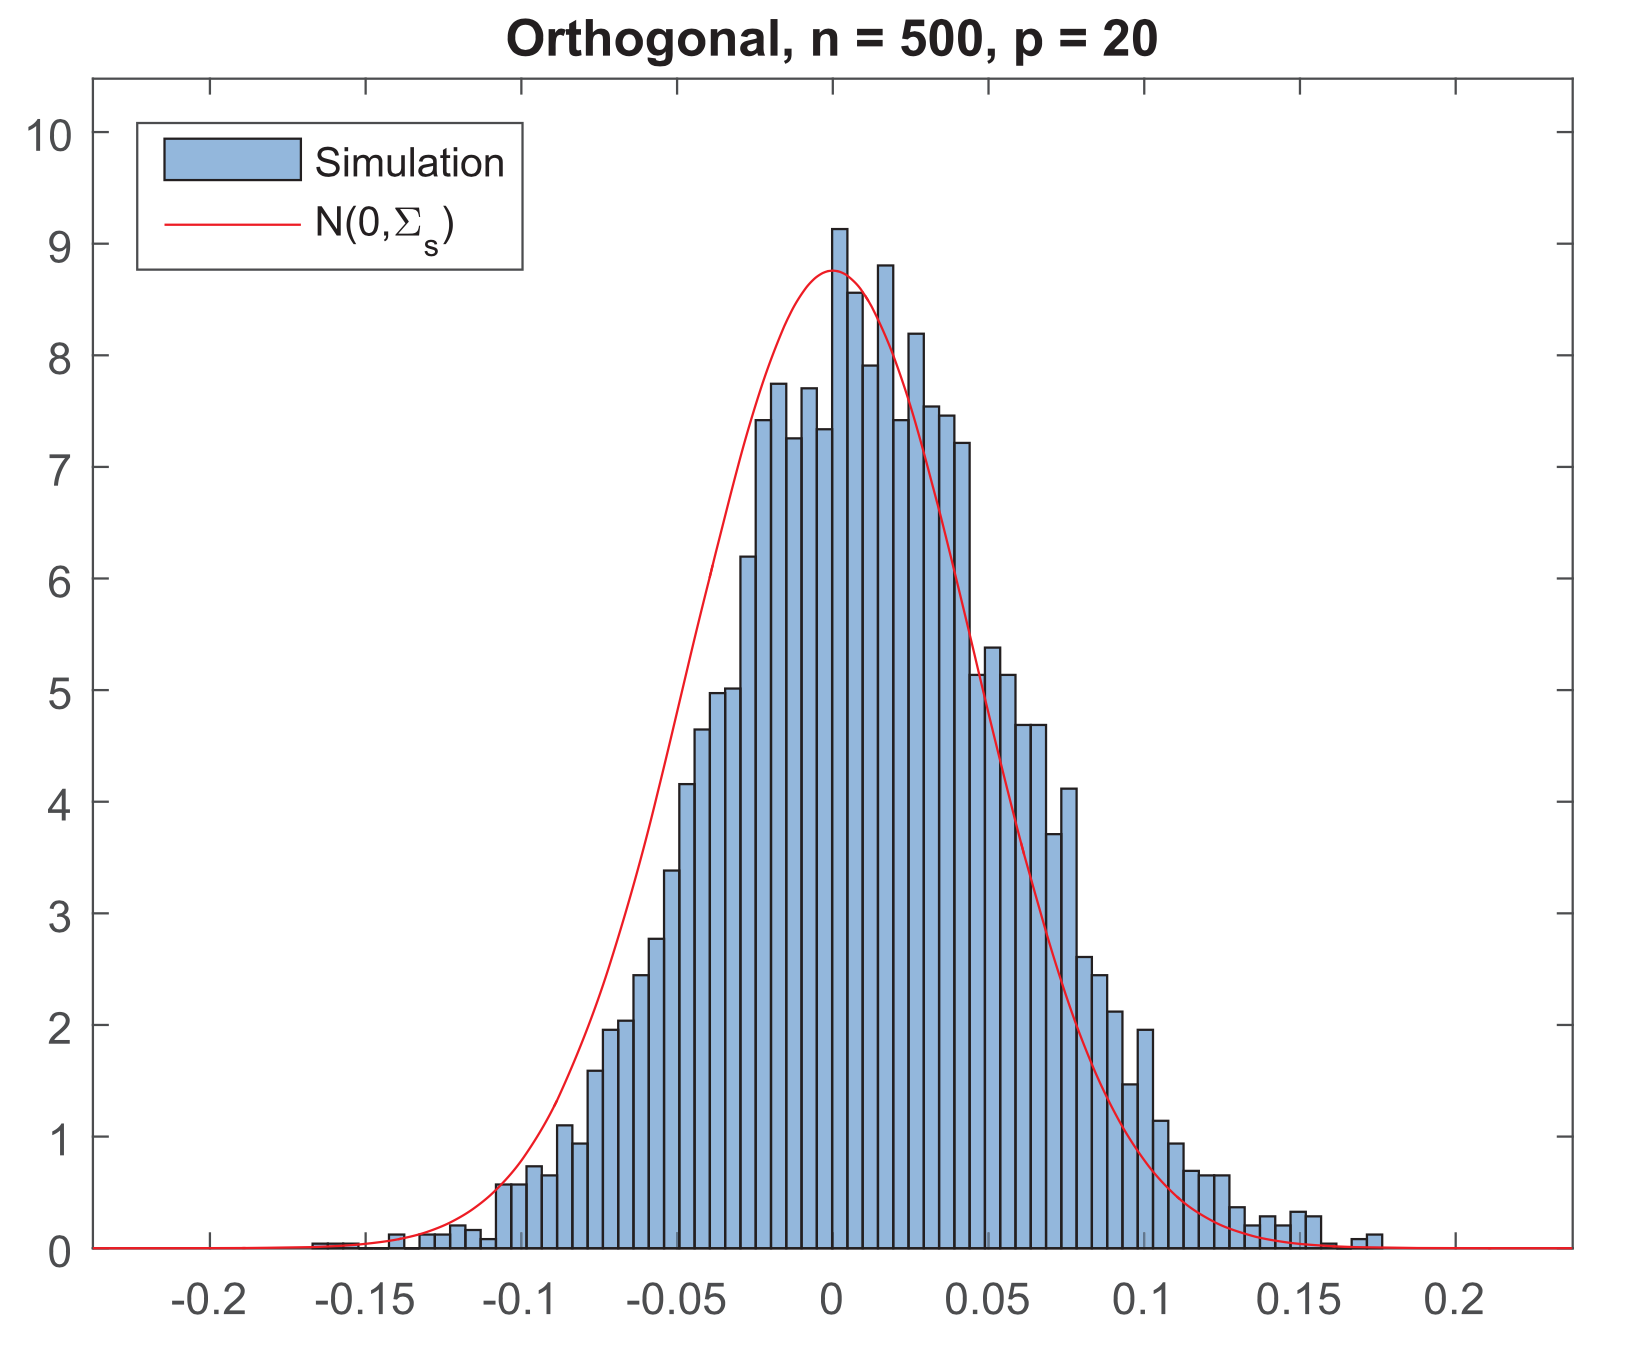
\includegraphics[width=0.6\textwidth]{fig/fig1b.png}
	\end{figure}

	\end{frame}

	\begin{frame}
	\frametitle{Split Sample}
	We need to use independent sample sets for implementing 
	\begin{enumerate}
	\item Estimation for residuals $\hat{V}$ and $\hat{W}$
	\item Regression $\hat{W} $ on $\hat{V}$
	\end{enumerate}
	to get consistency.

	\end{frame}

	\begin{frame}
	\frametitle{Split Sample}
	\begin{figure}
	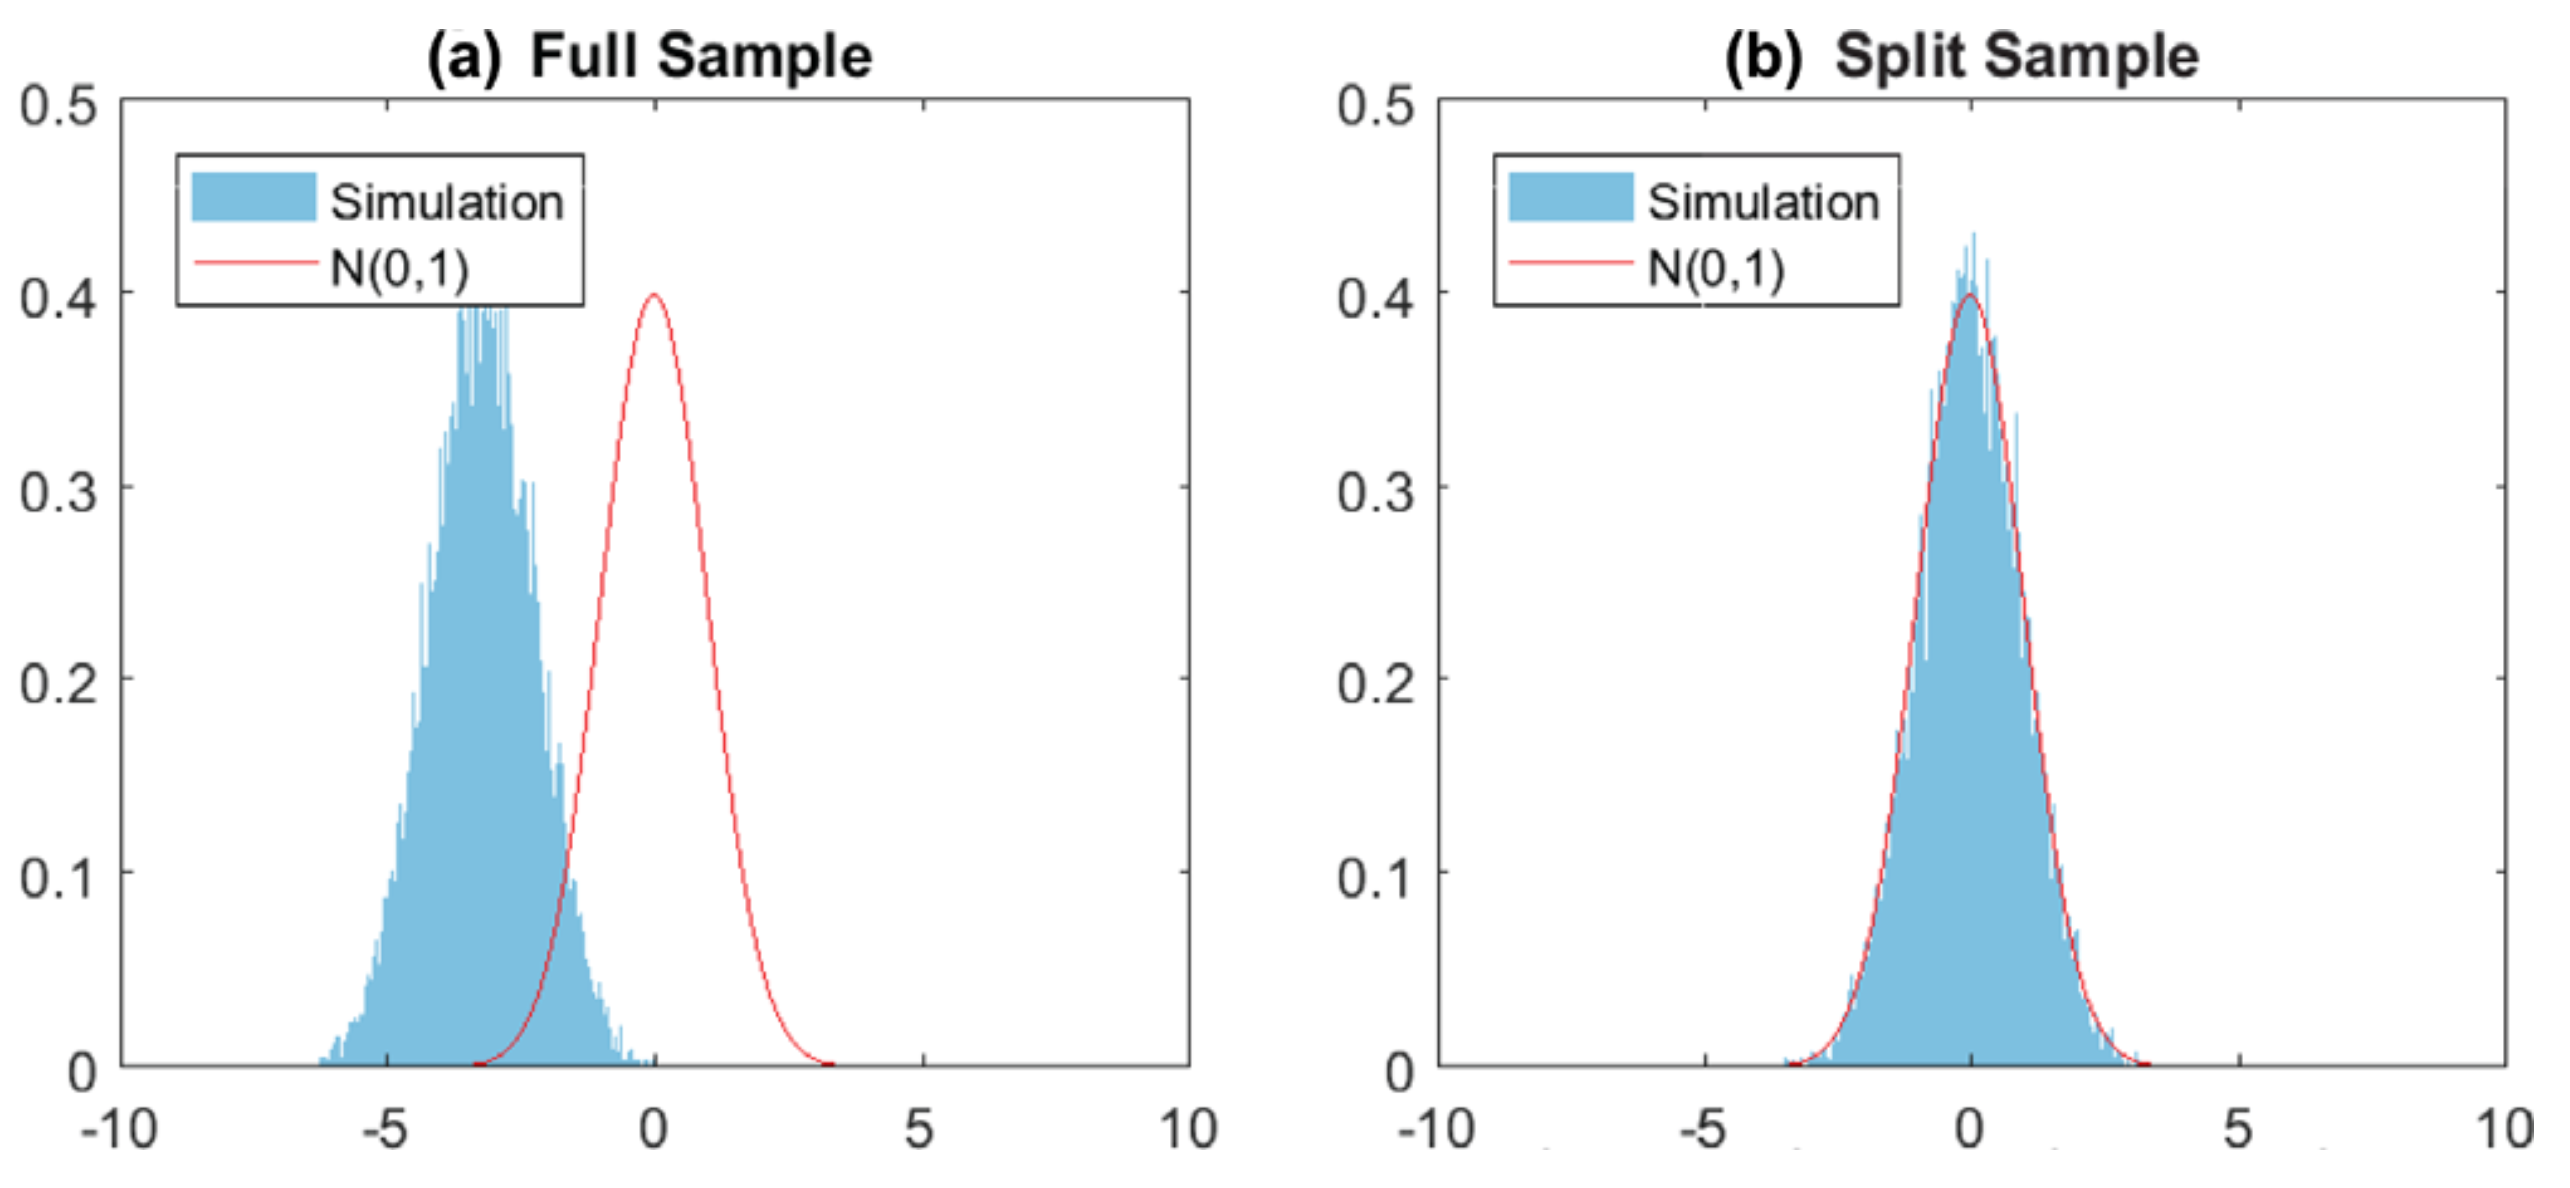
\includegraphics[width=0.9\textwidth]{fig/fig2.png}
	\end{figure}

	\end{frame}

	\begin{frame}
	\frametitle{Orthogonality: Non-linear Moment Condition}
	\begin{itemize}
	\item General non-linear moment condition:
	\begin{eqnarray*}
	E[\psi(W; \theta_0, \eta_0) ] = 0.
	\end{eqnarray*}
	\item In previous examples, $W=(Y,D,X) $ and $\eta_0 = (\beta_0,\gamma_0)$ or $(g_0,m_0)$.
	\item Orthogonality condition:
	\begin{eqnarray*}
	\partial_\eta E[\psi(W; \theta_0, \eta_0) ] = 0.
	\end{eqnarray*}
	\end{itemize}

	\end{frame}

	\begin{frame}
	\frametitle{Example: ATE}
	\begin{itemize}
	\item Consider
	\begin{eqnarray*}
	\begin{cases}
	Y = g_0(D,X) + U, & E[U|X,D]=0\\
	D = m_0(X) + V, & E[V|X]=0
	\end{cases}.
	\end{eqnarray*}
	\item Want to estimate ATE:
	\begin{eqnarray*}
	\theta_0 = E[g_0(1,X)-g_0(0,X)].
	\end{eqnarray*}
	\item Score can be $\psi(W; \theta, \eta) = $
	\begin{eqnarray*}
	(g(1,X)-g(0,X))+\frac{D(Y-g(1,X))}{m(X)}-\frac{(1-D)(Y-g(0,X))}{1-m(X)}-\theta,
	\end{eqnarray*}
	where $\eta = (g,m)$.
	\end{itemize}

	\end{frame}

	\begin{frame}
	\frametitle{Example: ATE}
	\begin{enumerate}
	\item Apply ML to predict $Y$ by $(D,X)$, and get $\hat{g}(D,X) $
	\begin{itemize}
	\item Caution: naive estimator $\hat{\theta} = \sum_{i=1}^N \left\{\hat{g}(1,x_i) - \hat{g}(0,x_i)\right\} $ will be biased!
	\end{itemize}
	\item Apply ML to predict $D$ by $X$, and get $\hat{m}(X) $
	\item DML estimator $\hat{\theta} = $
	\begin{eqnarray*}
	\sum_{i=1}^N \left\{(\hat{g}(1,x_i)-\hat{g}(0,x_i))+\frac{d_i(y_i-\hat{g}(1,x_i))}{\hat{m}(x_i)}-\frac{(1-d_i)(y_i-\hat{g}(0,x_i))}{1-\hat{m}(x_i)} \right\}
	\end{eqnarray*}
	is unbiased!!
	\begin{itemize}
	\item DML estimator coincides with the ``doubly robust'' estimator for ATE.
	\end{itemize}
	\end{enumerate}

	\end{frame}

	\begin{frame}
	\frametitle{Targeted minimum loss-based estimation (TMLE)}
	\begin{itemize}
	\item Variables
	\begin{itemize}
	\item $Y$: outcome
	\item $D$: treatment indicator
	\item $X$: covariates
	\end{itemize}
	\item Observe $(y_i,d_i,x_i) \sim P_0 $ i.i.d. for $i=1,\dots,N $
	\item Statistical model $\mathcal{M} $ contains $P_0 $
	\item Want to estimate $\Psi(P) $: e.g, ATE
	\begin{eqnarray*}
	\Psi(P) = E_P[E_P(Y|D=1,X) - E_P(Y|D=0,X)]
	\end{eqnarray*}
	\item Idea of TMLE:
	\begin{enumerate}
	\item Estimate $P_0$ by MLE with a correction term $\epsilon $ $\Rightarrow $ $P_{\hat{\epsilon}} $
	\item Plug $P_{\hat{\epsilon}} $ into estimator of $\Psi $ $\Rightarrow $ TMLE estimator $\hat{\Psi}(P_{\hat{\epsilon}}) $
	\end{enumerate}
	\item Also use sample splitting.
	\end{itemize}

	\end{frame}

	\begin{frame}
	\frametitle{Example: ATE}
	\begin{enumerate}
	\item Set statistical model: $P(Y|D,X) \sim \mathcal{N}(m(D,X),\sigma^2(D,X)) $
	\item Obtain correction formula: $P_\epsilon(Y|D,X) \sim \mathcal{N}(m(D,X) + \epsilon h(P)(D,X),\sigma^2(D,X)) $
	\begin{eqnarray*}
	\text{where } h(P)(D,X) = \left(\frac{\I(D=1)}{E_P[D=1|X]} - \frac{\I(D=0)}{E_P[D=0|X]} \right) \sigma^2(D,X)
	\end{eqnarray*}
	\begin{itemize}
	\item Correction is made to satisfy the ``efficient influence curve'' condition
	\end{itemize}
	\item Estimate $m(D,X),\sigma^2(D,X),\epsilon $ with MLE by fitting $P_\epsilon(Y|D,X) $ to data \\
	$\Rightarrow $ $\hat{m}(D,X),\hat{h}(D,X),\hat{\epsilon} $
	\item $\hat{m}(D,X) + \hat{\epsilon} \hat{h}(D,X)$ is the corrected estimator for $E_P(Y|D,X)$
	\item TMLE estimator
	\begin{eqnarray*}
	\hat{\Psi}(P_{\hat{\epsilon}}) = \sum_{i=1}^N \left[ \left\{\hat{m}(1,X) + \hat{\epsilon} \hat{h}(1,X) \right\} - \left\{\hat{m}(0,X) + \hat{\epsilon} \hat{h}(0,X) \right\} \right]
	\end{eqnarray*}
	\end{enumerate}

	\end{frame}

	\begin{frame}
	\frametitle{Difference between TMLE and DML?}
	\begin{itemize}
	\item van der Laan and D\'iaz argue TMLE is more general framework\\
	$\Rightarrow $ No, they ignore Chernozhukov et al. (2022), which provides a general framework of Chernozhukov et al. (2018)
	\item Both are coming from the semiparametric idea of first stage estimator can be high-dimensional when the second stage parameter of interest is low dimension.
	\item They are just following different contexts:
	\begin{itemize}
	\item Biostatistics, statistical model
	\item Econometrics, GMM
	\end{itemize}
	\end{itemize}
	\end{frame}

























\end{document}
